\section*{Exercice 177 -- Réducteur de roue motrice de chariot élévateur}
\setcounter{exo}{0}
 
\textit{D'après Florestan Mathurin.}
\setcounter{exo}{0}

\ifprof
\else

On s’intéresse au réducteur équipant la roue arrière motrice et directionnelle d’un chariot élévateur de manutention automoteur à conducteur non porté. 



\begin{center}
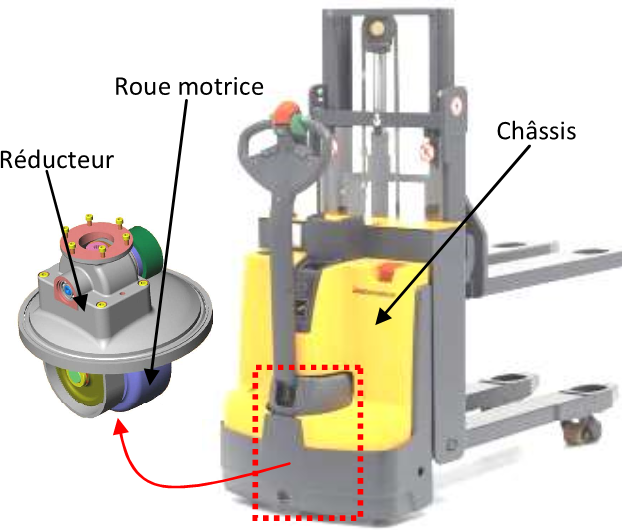
\includegraphics[width=.5\linewidth]{char_01}
\end{center}


\textbf{Données }: $z_{27} = \SI{16}{dents}$, $z_{35} = \SI{84}{dents}$, $z_{5} = \SI{14}{dents}$, $z_{11} = \SI{56}{dents}$, $z_{16} = \SI{75}{dents}$. 

\fi

\subparagraph{}
\textit{Identifier les classes d’équivalence cinématique sur le dessin d’ensemble. }
\ifprof
\begin{corrige}

\end{corrige}
\else
\begin{center}
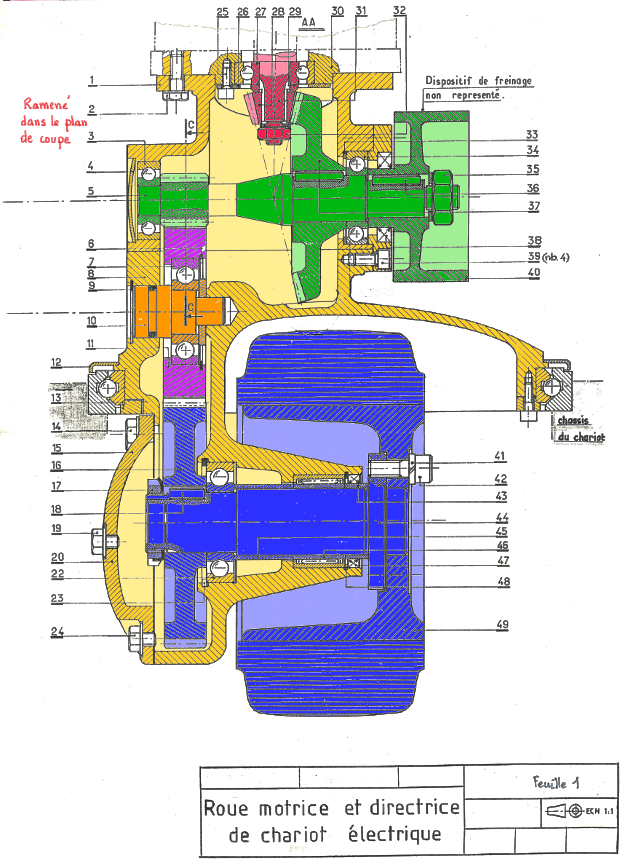
\includegraphics[width=\linewidth]{char_02}
\end{center}

\fi



\subparagraph{}
\textit{ Construire le schéma cinématique du réducteur dans le même plan que le dessin.}
\ifprof
\begin{corrige}
\begin{center}
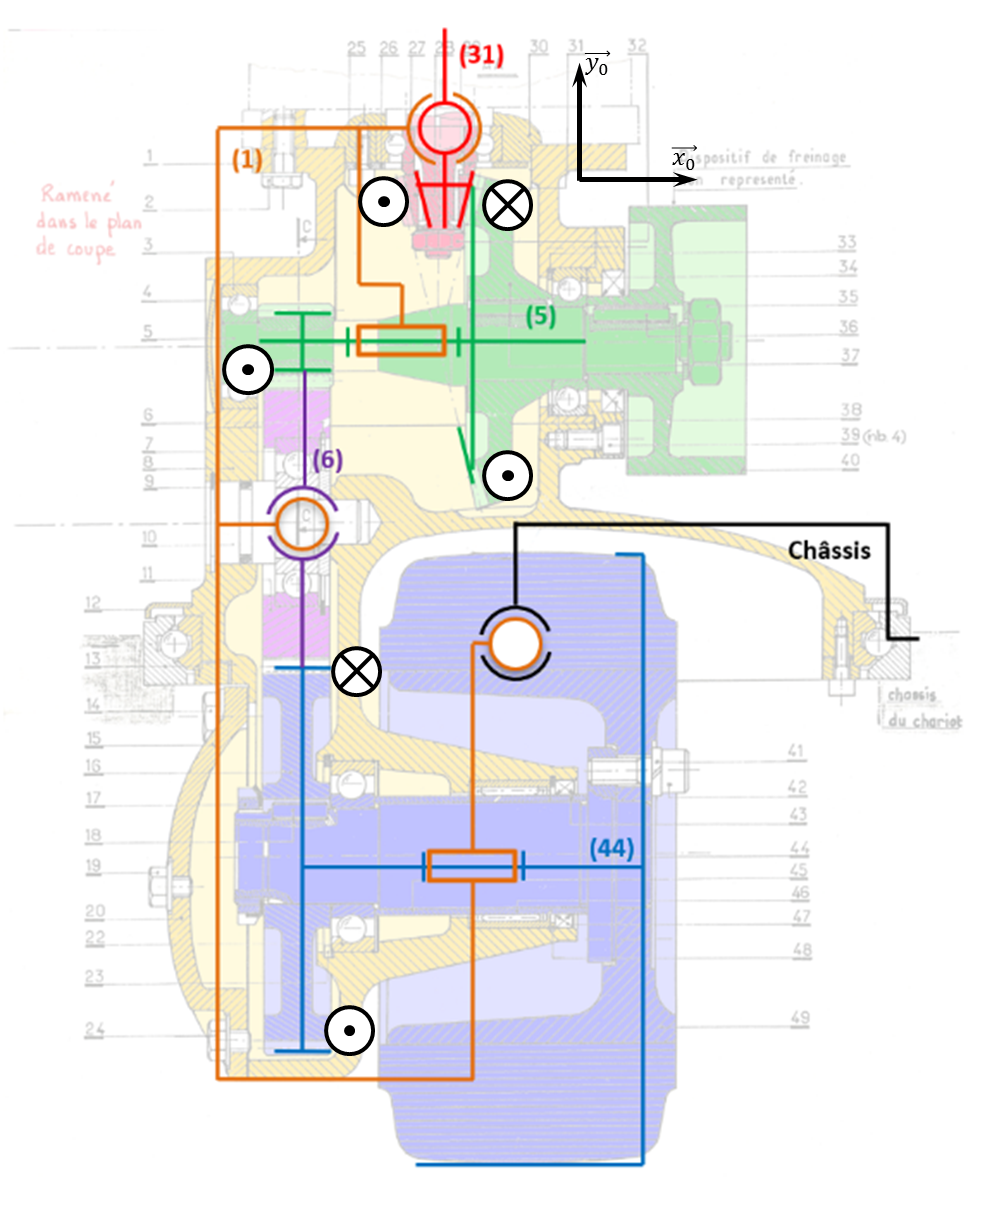
\includegraphics[width=\linewidth]{char_cor_01_BIS}
\end{center}
\end{corrige}
\else
\fi
\subparagraph{}
\textit{Compléter le tableau donnant les caractéristiques des roues et pignons.}
\ifprof
\begin{corrige}
\footnotesize
\begin{center}
\begin{tabular}{|c|c|c|c|}
\hline
Repère de  & Module  & Nombre & Diamètre primitif  \\
la roue & $m$ (mm) & de dents $Z$ & $D$ (mm) \\
\hline
\hline
27 & 1,5 &16 & 24\\ \hline
35 & 1,5 &84 & 126\\ \hline
5   &1,5 &14 & 21\\ \hline
11 & 1,5 & 56 & 84 \\ \hline
16 &  1,5&  75& 112,5\\ \hline

\end{tabular}
\end{center}

\normalsize
\end{corrige}
\else
\footnotesize
\begin{center}
\begin{tabular}{|c|c|c|c|}
\hline
Repère de  & Module  & Nombre & Diamètre primitif  \\
la roue & $m$ (mm) & de dents $Z$ & $D$ (mm) \\
\hline
\hline
27 & & & \\ \hline
35 & 1,5& & \\ \hline
5& & & \\ \hline
11& 1,5 & & \\ \hline
16& & & \\ \hline

\end{tabular}
\end{center}

\normalsize
\fi



\subparagraph{}
\textit{Après avoir proposé un paramétrage, indiquer dans quel sens tourne la roue si le moteur 28 (31) tourne dans le sens positif.}

\ifprof
\begin{corrige}
Voir figure précédente. Si le moteur tourne dans le sens positif, la roue tourne dans le sens négatif. 
\end{corrige}
\else
\fi

\subparagraph{}
\textit{Pour une vitesse de \SI{1500}{tr/min} en sortie de moteur, déterminer la vitesse de rotation de la roue. Le diamètre de la roue est de \SI{150}{mm}. Quelle est la vitesse du véhicule ? }
\ifprof
\begin{corrige}
Le rapport de réduction de la transmission est le suivant : 
$k=\dfrac{Z_{27} Z_{5} Z_{11} }{Z_{35} Z_{11} Z_{16}} = \dfrac{16\cdot 14}{84\cdot 75} =0,0355 $

La vitesse de rotation de la roue est donc de $\SI{53,33}{tr.min^{-1}}$ soit \SI{5,59}{rad.s^{-1}}. 
On en déduit la vitesse du véhicule : $5,59 \times 0,15 = \SI{0,84}{m.s^{-1}}\simeq \SI{3}{km.h^{-1}}$.

\end{corrige}
\else
\fi
